%!TEX root = Slic3r-Manual.tex

\section{Optimisation du Remplissage} % (fold)
\label{sec:infill_optimization}
\index{infill}
\index{remplissage}

Slic3r contient plusieurs param\`etres de remplissage avanc\'es qui peuvent aider \`a produire de meilleurs extrusions.

\begin{figure}[H]
\centering
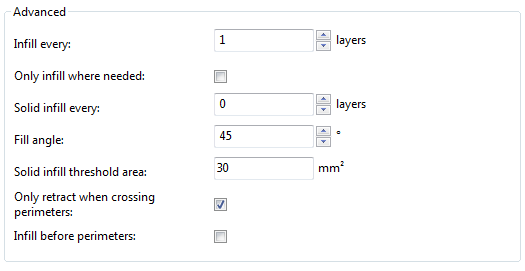
\includegraphics[keepaspectratio=true,width=1\textwidth]{expertmode/infill_advanced_settings.png}
\caption{Param\`etres avanc\'es de remplissage.}
\label{fig:infill_settings}
\end{figure}
\index{Print Settings!Infill!Infill every n layers}
\index{Param\`etres d'Impression!Remplissage!Remplissage tous les n couches}
\index{Print Settings!Infill!Only infill where needed}
\index{Param\`etres d'Impression!Remplissage!Remplissage uniquement si n\'ecessaire}
\index{Print Settings!Infill!Solid infill every n layers}
\index{Param\`etres d'Impression!Remplissage!Remplissage plein tous les n couches}
\index{Print Settings!Infill!Fill angle}
\index{Param\`etres d'Impression!Remplissage!Angle de remplissage}
\index{Print Settings!Infill!Solid infill threshold area}
\index{Param\`etres d'Impression!Remplissage!Seuil de l'aire de remplissage plein}
\index{Print Settings!Infill!Only retract when crossing perimeters}
\index{Param\`etres d'Impression!Remplissage!Retrait uniquement lors d'un croisement avec un p\'erim\`etre}
\index{Print Settings!Infill!Infill before perimeters}
\index{Param\`etres d'Impression!Remplissage!Remplissage avant les p\'erim\`etres}

\begin{itemize}
    \item \texttt{Infill every \textit{n} layers} (Remplissage tous les n couches) - Produira remplissage vertical \'eparse en sautant d'un certain nombre de couches. Ceci peut \^etre utilis\'e pour acc\'el\'erer le temps d'impression o\`u le remplissage manquant est acceptable.
    \item \texttt{Only infill where needed} (Remplissage uniquement si n\'ecessaire) - Slic3r analysera le mod\`ele et choisir l'endroit o\`u le remplissage est n\'ecessaire pour soutenir les plafonds internes et les surplombs. Utile pour la r\'eduction du temps et de l'utilisation de la mati\'ere.
    \item \texttt{Solid infill every \textit{n} layers} (Remplissage plein tous les n couches) - Force un motif de remplissage solide sur les couches sp\'ecifi\'ees. Z\'ero pour d\'esactiver cette option.
    \item \texttt{Fill angle} (Angle de remplissage) - Par d\'efaut, le motif de remplissage est orient\'e \`a 45 ° afin de fournir la meilleure adh\'erence aux structures des mur. Extrusions d'intercalaires qui courent \`a c\^ot\'e de p\'erim\`etres sont susceptibles de d\'e-stratifi\'e en situation de stress. Certains mod\`eles peuvent n\'ec\'eciter une rotation de l'angle de remplissage afin d'assurer la direction optimale de l'extrusion.
    \item \texttt{Solid infill threshold area} (Seuil de l'aire de remplissage plein) - Les petites surfaces dans le mod\`ele sont g\'en\'eralement mieux lotis \'etant compl\`etement rempli pour fournir l'int\'egrit\'e structurelle. Toutefois Cela prendra plus de temps et de mati\`ere, sans que la cette solidit\'ee soit n\'ecessaire. R\'eglez cette option s'adapter aux besoins.
    \item \texttt{Only retract when crossing perimeters} (Retrait uniquement lors d'un croisement avec un p\'erim\`etre) - La r\'etractation, pour emp\^echer le suintement, n'est pas n\'ecessaire si l'extrudeuse reste dans les limites du mod\`ele. Des pr\'ecautions doivent \^etre prises si la mati\`ere d'impression suinte trop, ne pas se r\'etracter peut entra\^iner la perte de mati\`ere assez qui affectera la qualit\'e de l'extrusion ult\'erieure. Cependant, la plupart des imprimantes modernes et des mati\`eres souffrent rarement de tels probl\`emes de suintentement extr\^emes.
    \item \texttt{Infill before perimeters} (Remplissage avant les p\'erim\`etres) - Inverse l'ordre dans lequel la couche est imprim\'ee. Habituellement, le p\'erim\`etre est fix\'e dans un premier temps, suivie duremplissage, ce qui est g\'en\'eralement pr\'ef\'erable tant le p\'erim\`etre joue le r\^ole d'une paroi contenant le remplissage.
\end{itemize}


% section infill_optimization (end)